De los 16 encuentros semanales en línea a lo largo del cuatrimestre en 13 de ellos se presentan nuevos temas. De estos se seleccionaron algunos para ilustrar la progresión del curso.

\textbf{Clase 1.} Repaso de la mecánica Newtoniana, el análisis y el álgebra requeridos para obtener la dinámica del péndulo ideal revisitando las aproximaciones y cálculos vistos en Física 1. Este material de teoría se distribuye tanto en esta como en las subsiguientes clases en un cuaderno Jupyter. Se anima a los alumnos a revisar la notación LaTeX con las que el docente escribe fórmulas matemáticas como las que se muestran en la figura \ref{fig:clase1pendulo}. 

\begin{figure}[!ht]
\centering
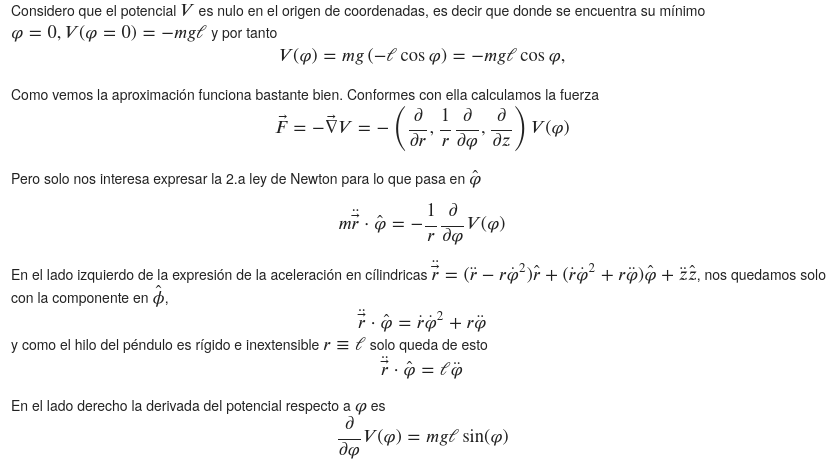
\includegraphics[width=3.5in]{figuras/clase1péndulo.png}
\caption{La teoría se presenta en cuadernos Jupyter. Todos las fórmulas matemáticas se expresan en notación estandarizada \LaTeX que los alumnos pueden editar o copiar para sus propios fines.}
\label{fig:clase1pendulo}
\end{figure}

En adición a la reiteración de lo ya visto en cursos anteriores en esta primera clase ya se avanza en el uso de código para analizar resultados. La figura \ref{fig:clase1graficos} muestra instrucciones para que la biblioteca Matplotlib grafique la solución para la dinámica del péndulo ideal.

\begin{figure}[!ht]
\centering
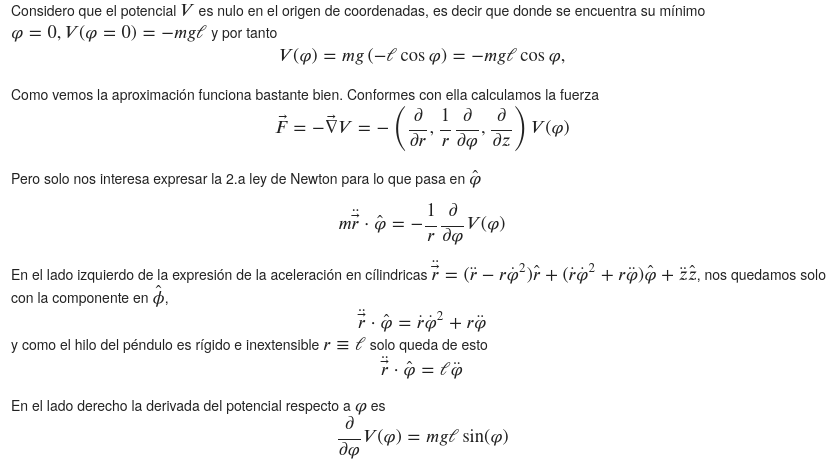
\includegraphics[width=3.5in]{figuras/clase1péndulo.png}
\caption{Desde la primera clase se hace explícito a los estudiantes el código utilizado para el análisis de sistemas. Aquí las funciones de Matplotib para graficar la dinámica de un péndulo ideal.}
\label{fig:clase1graficos}
\end{figure}

\textbf{Clase 3.} A partir de esta clase se aplica en clase la biblioteca Sympy para el cálculo simbólico automático. La figura \ref{fig:clase3sympy} muestra cómo para calcular la energía cinética de un sistema con dos coordenadas generalizadas se diferencia en su sistema de referencia.

\begin{figure}[!ht]
\centering
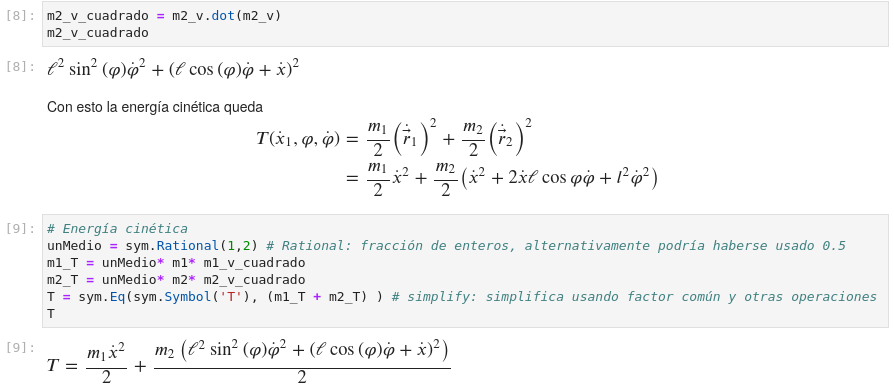
\includegraphics[width=3.5in]{figuras/clase3sympy.png}
\caption{Primeros cálculos simbólicos utilizando la biblioteca SymPy.}
\label{fig:clase3sympy}
\end{figure}

\textbf{Clase 4.} Las ecuaciones de Euler-Lagrange permiten a los alumnos obtener las ecuaciones que describen la dinámica de un sistema. La figura \ref{fig:clase4euler} muestra como funciones de la biblioteca Sympy facilitan el obtener tales ecuaciones para un sistema de dos grados de libertad.

\begin{figure}[!ht]
\centering
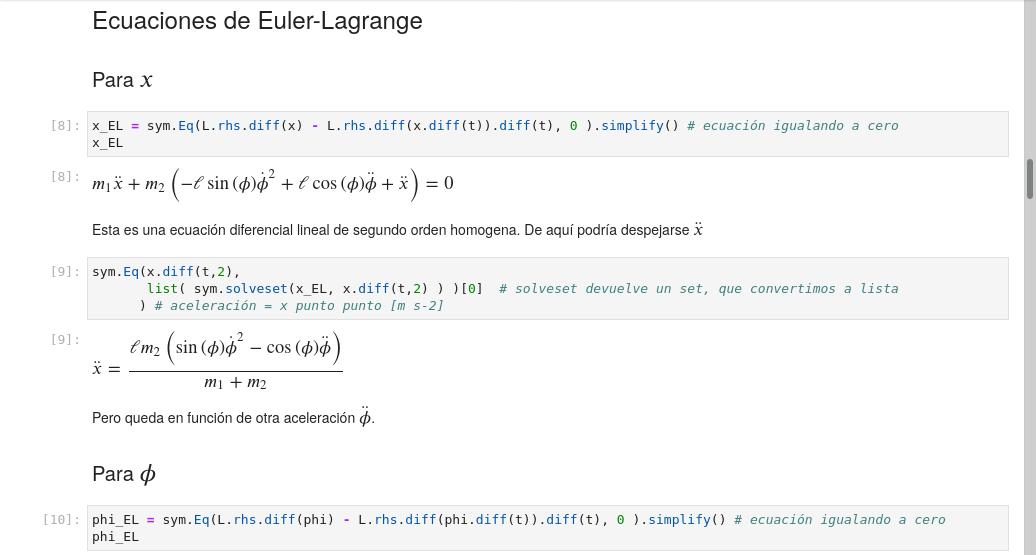
\includegraphics[width=3.5in]{figuras/clase5EulerLagrange.png}
\caption{Aplicación de funciones de SymPy para general las ecuaciones diferenciales de Euler-Lagrange que describen la dinámica de un sistema.}
\label{fig:clase4euler}
\end{figure}

Hasta aquí se ha utilizado el código para realizar los mismos pasos que en un curso de mecánica racional convencional se resuelven en pizarrón o papel para arribar a ecuaciones diferenciales que solo se resuelven para casos triviales. En contrapartida utilizando Sympy se resuelven rápidamente sistemas complejos para aceleraciones en función de coordenadas y velocidades generalizadas como se muestra en la figura \ref{fig:clase4ac}. Realizar tal tarea manualmente insumiría un tiempo y esfuerzo no despreciable inclusive para este sistema con meros dos grados de libertad.

\begin{figure}[!ht]
\centering
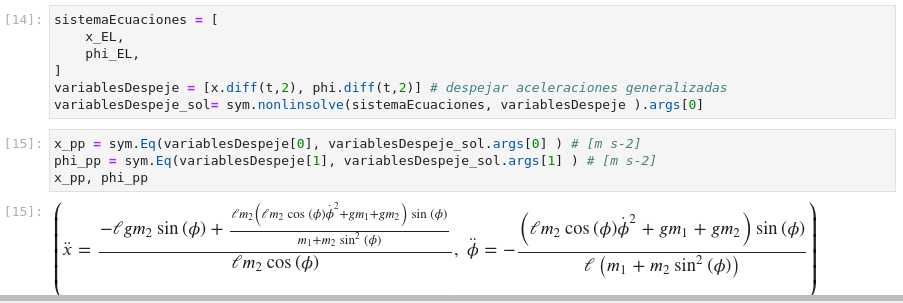
\includegraphics[width=3.5in]{figuras/clase4Aceleraciones.png}
\caption{La resolución de sistemas de ecuaciones diferenciales de cierta complejidad se evita en cursos convencionales. En este curso solo insume un par de líneas de código con funciones de la biblioteca Sympy.}
\label{fig:clase4ac}
\end{figure}

\textbf{Clase 5.} Los estudiantes aprobaron un curso de cálculo numérico para poder inscribirse a este curso en el que se hará uso de tales conocimientos. En clase se repasan los fundamentos de los métodos de resolución numérica de ecuaciones diferenciales y cómo se implementarían en una notación de vectores de estado adecuada para un eficiente procesamiento. Tal repaso se presenta a los estudiantes con la misma metodología que para los otros temas, en cuadernos Jupyter que los alumnos pueden editar, como se muestra en la figura \ref{fig:clase5res}.  

\begin{figure}[!ht]
\centering
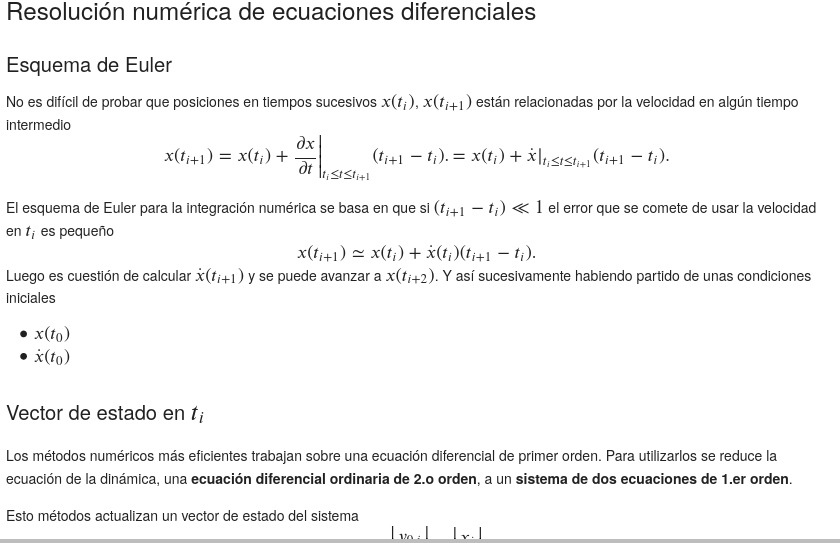
\includegraphics[width=3.5in]{figuras/clase5Euler.png}
\caption{Previo a proceder a la resolución numérica de ecuaciones diferenciales se presenta, en cuadernos de Jupyter, un repaso de sus fundamentos.}
\label{fig:clase5res}
\end{figure}

Inmediatamente tras el repaso de fundamentos se muestran en acción las funciones de la biblioteca de cálculo científico Scipy para obtener eficientemente las soluciones para la dinámica de un sistema de dos grados de libertad como se ilustra en la figura \ref{fig:clase5sol}.

\begin{figure}[!ht]
\centering
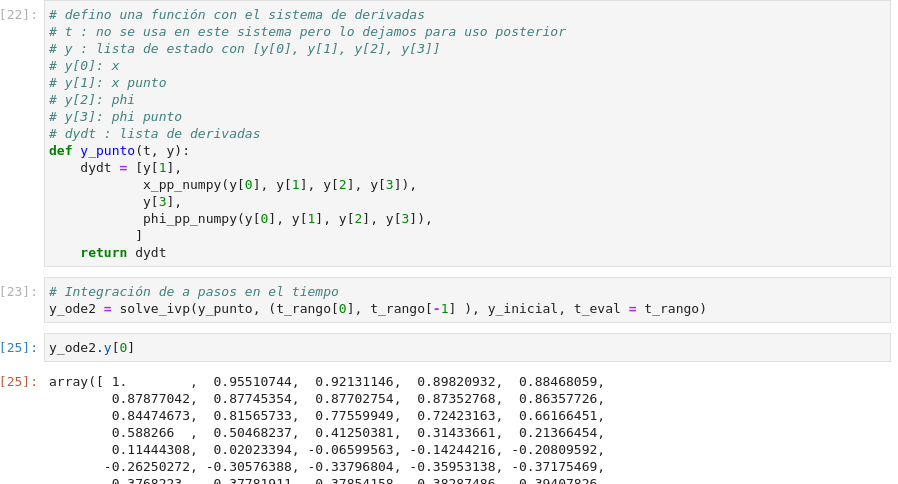
\includegraphics[width=3.5in]{figuras/clase5Soluciones.png}
\caption{Se resuelve numéricamente el sistema de ecuaciones para la dinámica de un sistema de dos grados de libertad con funciones de la biblioteca SciPy.}
\label{fig:clase5sol}
\end{figure}

Las posiciones y velocidades generalizadas en el rango de tiempos de interés obtenidas numéricamente se representan gráficamente. La figura \ref{fig:clase5rep} muestra tal representación que sirve para discutir con los alumnos si el comportamiento del sistema se condice con el que puede predecirse de un análisis cualitativo de este sistema simple. El comprobar que las herramientas utilizadas de cálculo simbólico y numérico obtienen resultados correctos confiere confianza en los mismos en vistas de aplicarles a sistemas más complejos.

\begin{figure}[!ht]
\centering
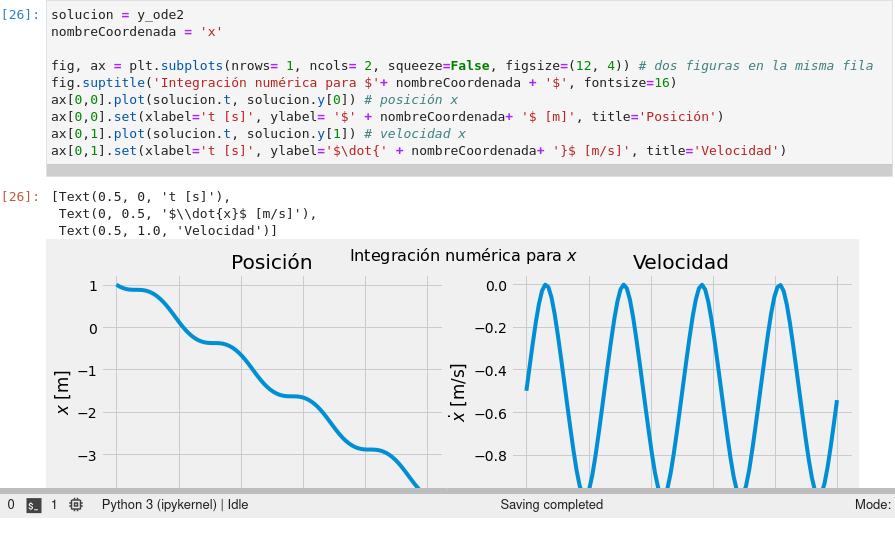
\includegraphics[width=3.5in]{figuras/clase5Representación.png}
\caption{Visualización de resultados obtenidos por cálculo numérico. Corroborando que lo representado corresponde con un análisis cualitativo de la dinámica del sistema se crea confianza en los alumnos en esta herramienta.}
\label{fig:clase5rep}
\end{figure}

\subsection{Clase 7.} Se incorpora a los códigos el análisis de fuerzas no conservativas que a fin de cuentas son la mayoría de las que pueden afectar a un dispositivo mecánico industrial. Como primer ejemplo se extiende la analogía de las oscilaciones del péndulo a un sistema amortiguado que se muestra en la figura \ref{fig:clase7esquema}.

\begin{figure}[!ht]
\centering
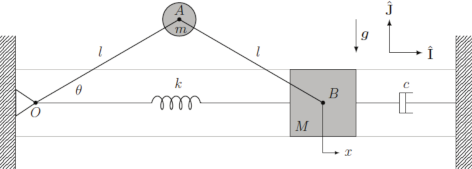
\includegraphics[width=3.5in]{figuras/clase7esquema.png}
\caption{Paulatinamente se extiende el rango de factores analizables. En este sistema actúa un amortiguador lineal con la velocidad. Esta fuerza no conservativa no podía analizarse con el código de clases precedentes.}
\label{fig:clase7esquema}
\end{figure}

La figura \ref{fig:clase7amo} muestra la gráfica que permite analizar la dinámica calculada con el mismo procedimiento y código que se viene utilizando en las clases precedentes.

\begin{figure}[!ht]
\centering
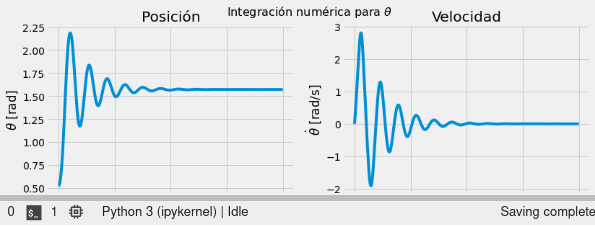
\includegraphics[width=3.5in]{figuras/clase7amortiguado.png}
\caption{Paulatinamente se extiende el rango de factores analizables. En este sistema actúa un amortiguador lineal con la velocidad. Esta fuerza no conservativa no podía analizarse con el código de clases precedentes.}
\label{fig:clase7amo}
\end{figure}

\textbf{Siguientes clases.} El temario habitual de un curso de mecánica racional se va completando centrándose en sistemas extensos analizados en el marco del cuerpo rígido y el análisis de oscilaciones forzadas en sistemas de múltiples grados de libertad. Hacia finales del curso los alumnos ya han desarrollado la habilidad de analizar en forma autónoma sistemas “realistas” en términos de ser más semejantes a dispositivos mecánicos existentes en la industria. Para plasmar esto último se les propone que calculen los torques que deben realizar los motores de un muy simplificado brazo robótico industrial para que este realice una secuencia de movimientos. Ejemplos del resultado del trabajo de alumnos en respuesta a esta propuesta se muestran en la figura \ref{fig:robotarm}.

\begin{figure}[!ht]
\centering
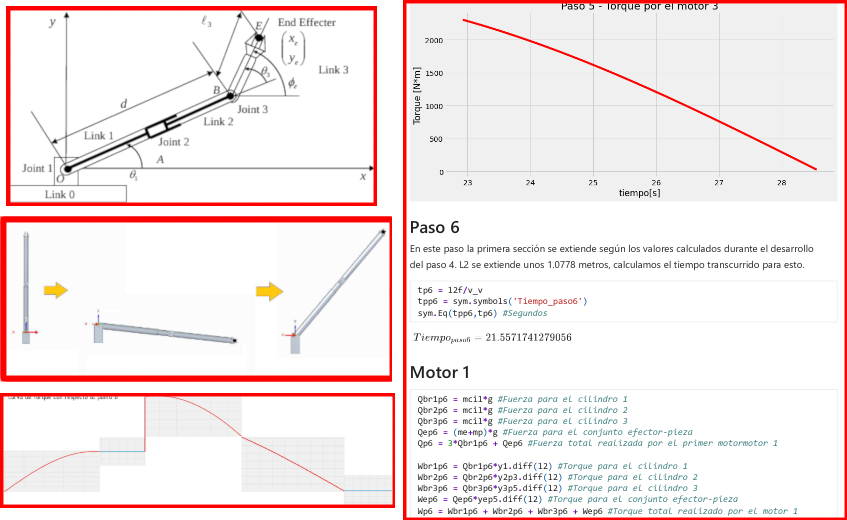
\includegraphics[width=3.5in]{figuras/robotArm.png}
\caption{Para que un brazo mecánica industrial  realice aún un simple movimiento se requiere que sus motores apliquen una secuencia de torques. Los alumnos realizan el cálculo de los mismos en un trabajo que plasma su dominio de las herramientas analíticas e informáticas cuyo uso fue aprendido en el curso.}
\label{fig:robotarm}
\end{figure}